% Copyright (C) 2005-2015 Airbus - EDF - IMACS - Phimeca
% Permission is granted to copy, distribute and/or modify this document
% under the terms of the GNU Free Documentation License, Version 1.2
% or any later version published by the Free Software Foundation;
% with no Invariant Sections, no Front-Cover Texts, and no Back-Cover
% Texts.  A copy of the license is included in the section entitled "GNU
% Free Documentation License".
\renewcommand{\filename}{docUC_StocProc_ARMA_Manipulation.tex}
\renewcommand{\filetitle}{UC : Manipulation of an ARMA process}

% \HeaderNNIILevel
% \HeaderIILevel
\HeaderIIILevel

\label{ARMAManipulation}

\index{Stochastic Process!ARMA}

Once an $ARMA(p,q)$ model has been created, it is possible to get :
\begin{itemize}
\item  its linear recurrence thanks to the method \emph{print},
\item  its AR and MA coefficients thanks to the methods \emph{getARCoefficients, getMACoefficients},
\item  its white noise thanks to the method \emph{getWhiteNoise}, that contains the time grid of the process,
\item  its current state, that is its last $p$ values and the last $q$ values of its white noise,  thanks to the method \emph{getState},
\item   a realization thanks to the method \emph{getRealization},
\item  a sample of realizations thanks to the method \emph{getSample},
\item  a possible future of the model, which is a possible prolongation of the current state on the next $n_{prol}$ instants, thanks to the method \emph{getFuture}.
\item   $n$ possible futures of the model, which correspond to  $n$ possible prolongations of the current state on the next $n_{prol}$ instants, thanks to the method \emph{getFuture}($n_{prol}$, $n$).
\end{itemize}


It is important to note that :
\begin{itemize}
\item when asking for a \emph{realization} of the stationary process modeled by $ARMA(p,q)$, one has to obtain a realization that does not depend on the current state of the process;
\item whereas, when one asks for a \emph{possible future} extending a particular curent state of the process, the realization of the model must depend on that current sate.
\end{itemize}

How to proceed to respect these constraints?\\
If we note $\vect{X}_1(\omega,t)$ and  $\vect{X}_2(\omega,t)$ two distinct solutions of (\ref{dimn}) associated to two distinct intial states, then, the process $\vect{D}(\omega,t) = \vect{X}_2(\omega,t) - \vect{X}_1(\omega,t)$ is solution of the homogeneous equation associated to  (\ref{dimn}) and then decreases with time under the condition (\ref{Modul}). Let us note  $N_{ther}$ the number such that :
\begin{equation}\label{nTher}
  \left( \max_{i,j} |r_{ij}| \right)^{N_{ther}} < \varepsilon ,\Longleftrightarrow N_{ther} > \displaystyle \frac{\ln  \varepsilon}{\ln \max_{i,j} |r_{ij}|}
\end{equation}
where  the $r_i$ are the roots of the polynomials (\ref{PolPhi}) and  $\varepsilon$ is the precision of the computer ( $\varepsilon =2^{-53} \simeq 10^{-16}$). Then, after $N_{ther}$ instants, the process  $\vect{D}(\omega,t)$ has disappeared, which means that the processes  $\vect{X}_1(\omega,t)$ and  $\vect{X}_2(\omega,t)$ do not differ any more. As a conclusion, after  $N_{ther}$ instants, the realization of the ARMA process does not depend any more on the initial state.\\
That is why, when making a realization of the ARMA model, OpenTURNS makes a \emph{thermalization step} that simply consists in realizing the model upon $N_{ther}$ additional instants, erasing the $N_{ther}$ first values and finally only retaining the other ones. That step ensures that the realization of the process does not depend on the intial state.  \\
By default, the number  $N_{ther}$ is evaluated according to (\ref{nTher}) by the method  \emph{computeNThermalization}. The User could get access to it with the method \emph{getNThermalization} and can change the value with the method \emph{setNThermalization}. (In order to give back to $N_{ther}$ its default value, it is necessary to re-use the method  \emph{computeNThermalization}).\\

On the contrary, in the context of getting a possible future from a specified current state, the User should care that the number of additional instants $N_{it}$ on which he wants to extend the process, is such that $N_{it} <  N_{ther}$ because beyond $N_{ther}$, the future has no link with the present.\\
More precisely, after $N_{it}^*$ instants, such that :

\begin{equation}\label{nitEt}
  \left( \max_{i,j} |r_{ij}| \right)^{N_{it}^*} <  \max_{i} \sigma_i, \Longleftrightarrow N_{ther} > \displaystyle \frac{\max_{i} \sigma_i}{\ln \max_{i,j} |r_{ij}|}
\end{equation}

where the $\sigma_i$ are the components of the covariance matrix of the white noise $\vect{\varepsilon}$,  the influence of the initial state is of same order than the influence of the white noise.\\


Let us note that when the ARMA model is created whithout specifying the current state, Open TURN automatically proceeds to a  thermalization step at the creation of the ARMA object. \\
Before asking for the generation of a possible futur, the User has to specify the current state of the ARMA model, thanks to the creation method that takes into account the current state. In that case, OpenTURNS does not proceed to the thermalization step.\\

As an ARMA model is a stochastic process, the object \textit{ARMA} inherits the methods of the \textit{Process} object. Thus, it is possible to get its marginal processes, its time grid, its dimension and to get several realizations at a time of the process.\\




\requirements{

  \begin{description}
  \item[$\bullet$] an ARMA process {\itshape myARMA}
  \item[type:]  ARMA
  \end{description}

}
{

  \begin{description}
  \item[$\bullet$] the AR and MA coefficients : {\itshape myARCoef, myMACoef}
  \item[type:]  ARMACoefficients
  \end{description}

  \begin{description}
  \item[$\bullet$] an ARMAState {\itshape myARMAState}
  \item[type:]  ARMAState
  \end{description}

  \begin{description}
  \item[$\bullet$] the last realizations : {\itshape $myLastValues, myLastNoiseValues$}
  \item[type:]  NumericalSample
  \end{description}

  \begin{description}
  \item[$\bullet$] a white noise : {\itshape myWhiteNoise}
  \item[type:]  WhiteNoise
  \end{description}

  \begin{description}
  \item[$\bullet$] a time series : {\itshape ts}
  \item[type:]  TimeSeries
  \end{description}
}

\textspace\\
Python script for this Use Case :

\inputscript{script_docUC_StocProc_ARMA_Manipulation}

\textspace\\
The example illustrated  below is a 1D ARMA process with $p = 4$, $q=0$ with the following coefficients :
\begin{align*}
  X_t + 0.4X_{t-1} + 0.3X_{t-2} + 0.2X_{t-3} + 0.1X_{t-4} = \varepsilon_{t}
\end{align*}
The $\varepsilon$ considered is a Normal white noise with $\sigma = 0.01$. This process is stationary.\\

Figures (\ref{arma_Realization}) to (\ref{arma_Predictions}) respectively draw the graphs of one realization of the stationary process, a sample of 5 realizations of the process, one then 5  possible futures from the first realization on the next 50 instants (let us note that the thermalization number according to (\ref{nTher}) is 75 greater than 50).


\begin{figure}[H]
  \begin{minipage}{9cm}
    \begin{center}
      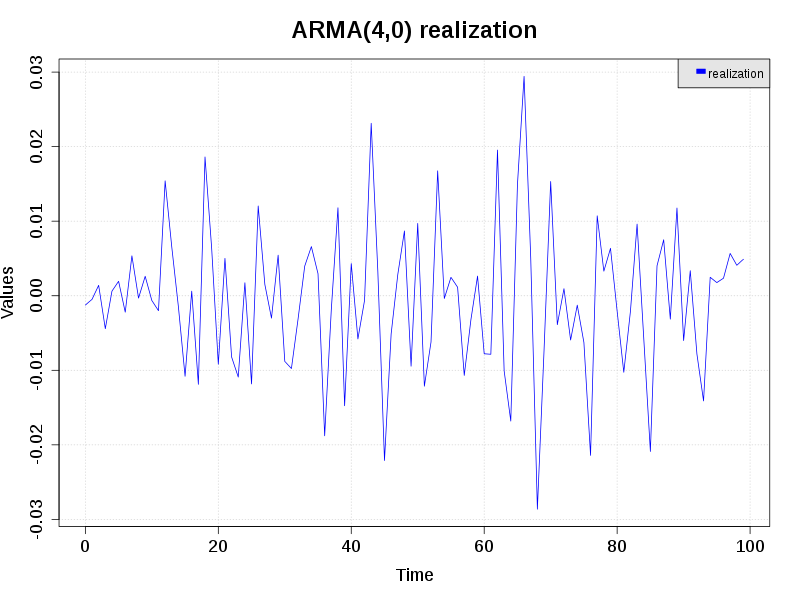
\includegraphics[width=7cm]{Figures/arma1D_realization.png}
      \caption{One realization of ARMA(4,0).}
      \label{arma_Realization}
    \end{center}
  \end{minipage}
  \hfill
  \begin{minipage}{9cm}
    \begin{center}
      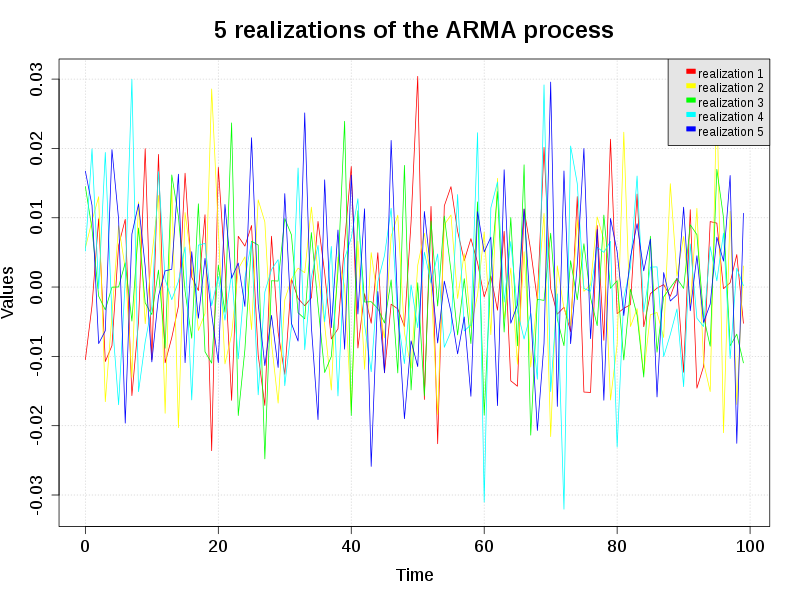
\includegraphics[width=7cm]{Figures/arma1D_realizations.png}
      \caption{$5$ realizations of ARMA(4,0).}
      \label{arma_Realizations}
    \end{center}
  \end{minipage}
\end{figure}


\begin{figure}[H]
  \begin{minipage}{9cm}
    \begin{center}
      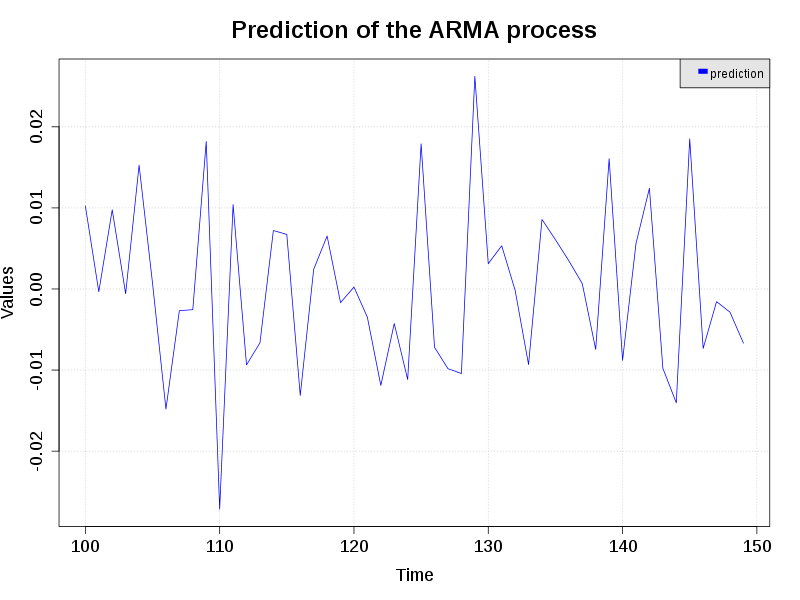
\includegraphics[width=7cm]{Figures/arma1D_prediction.png}
      \caption{One possible future of ARMA(4,0) on the next 50 instants.}
      \label{arma_Prediction}
    \end{center}
  \end{minipage}
  \hfill
  \begin{minipage}{9cm}
    \begin{center}
      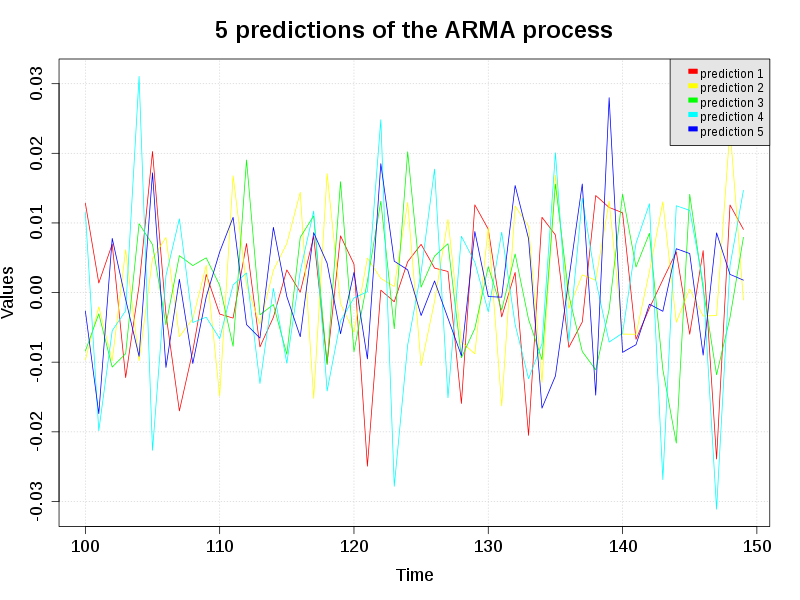
\includegraphics[width=7cm]{Figures/arma1D_predictions.png}
      \caption{$5$ possible futures of ARMA(4,0) on the next 50 instants.}
      \label{arma_Predictions}
    \end{center}
  \end{minipage}
\end{figure}
